\chapter{Verwendete Technologien}
\section{Git und GitHub}
Um als Team dynamisch arbeiten zu können, verwenden wir Software zur Versionsverwaltung. Hierbei handelt es sich um Git. 
Github ist die verwendete Online-Plattform, auf der Benutzer ihre Projekte als Repository hosten können. Dies ermöglicht einfaches arbeiten im Team und verhindert in den meisten Fällen Zusammenführungskonflikte. Mittels Git lässt sich auch einfach zurückverfolgen welches Teammitglied welche Änderungen gemacht hat. Bei Bedarf ist es möglich diese Änderungen zurückzusetzen.

Verwendet wird GitHub für die gesamte Diplomarbeit, sowohl für die Versionsverwaltung der Dokumente, als auch die einzelnen Applikationen. Um sicherzustellen, dass keine Konflikte durch paralleles Arbeiten entstehen, wird in Branches gearbeitet. Diese Branches wurden erstellt, wenn ein neues Arbeitspaket begonnen wurde, zum Beispiel die Android-App.

\begin{figure}[H]
\centering
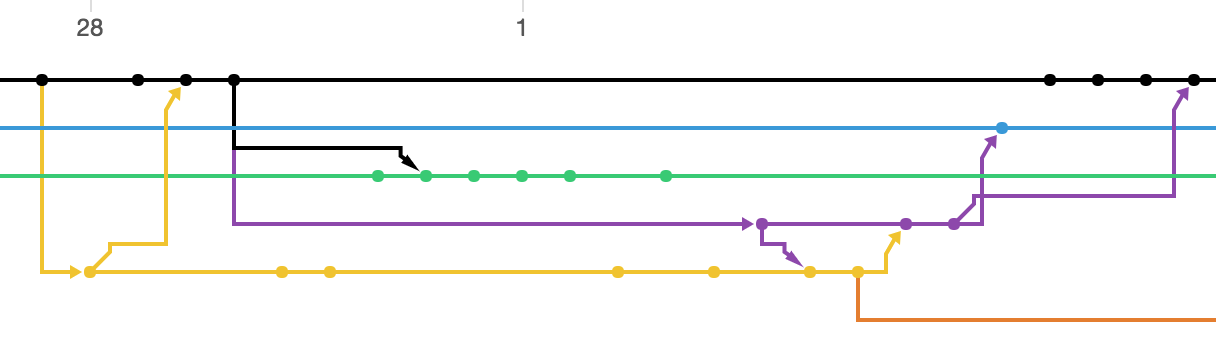
\includegraphics[width=1\textwidth]{images/04_VerwendeteTechnologien/network.png}
\caption{Github - Repository Network Diagramm}
\label{img:githubnetwork}
\end{figure}


\section{Android}

Android ist ein Betriebssystem für mobile Endgeräte, spezialisiert auf Touch-Anwendungen. Ziel ist es das Endgerät möglichst intuitiv und flexibel bedienen zu können. Mit Android ist es möglich open-source Applicationen zu erstellen, welche ein großes Publikum erreichen. Google stellt hier seinen eigenen ''PlayStore'' zur Verfügung, in dem die Applikationen gratis oder auch gegen Entgelt erworben werden können.
Diese Aspekte open-source, frei erhältlich und das Erreichen großes Publikum, sind ausschlaggebend dafür, dass die Applicationen in Android implementiert wird. Als Programmiersprache wird Java verwendet.
\\
\section{Java Enterprise Edition}\label{sec:javaee}
Die Java Platform, Enterprise Edition oder abgekürzt auch Java EE ist die technische nähere Beschreibung einer Softwarearchitektur, die programmierte Java Anwendungen ausführt. JavaEE baut auf JavaSE auf und ist dafür entwickelt worden um zuverlässige, sichere und skalierbare Netzwerkanwendungen erstellen zu können. \cite{differenceeese}\cite{wikijavaee}

\section{JSF - Java Server Faces}\label{sec:javaee}
JSF ist ein Java Enterprise Edition Framework, welches zur Entwicklung von Webanwendungen verwendet wird. JSF wurde als Nachfolger von JSP eingeführt um die Mischung von HTML Code und Java Code übersichtlicher zu gestalten. Ziel der JSF Vorgehensweise ist es Anwendungen in Komponenten zu teilen, welche im besten Fall wiederverwendbar sind. \cite{wikijsf}

\section{IntelliJ IDEA}
Herausgeber dieser Entwicklungsumgebung ist JetBrains. Durch diese IDE wird die Entwicklung des Java-EE-Backends unterstützt, wobei Java nicht die einzige Programmiersprache ist, die in IntelliJ verwendet werden kann. Andere Programmiersprachen, wie zum Beispiel Groovy und Kotlin, können in der IDE ebenfalls programmiert werden. Des weiteren gibt es eine Vielzahl an Tools wie zum Beispiel der direkte Zugang zu diversen Datenbanken, beispielsweise wie MySQL Datenbanken, oder die Integration von ''build automation tools'' wie bower oder grunt. Zudem sind verschiedenste Versionsverwaltungssysteme wie GutHub mit IntelliJ kompatibel und ebenfalls direkt über die Benutzeroberfläche der IDE verwendbar.\cite{wikiintelij}

\section{Android Studio}
Android Studio ist eine von Google und JetBrains bereitgestellte integrierte Entwicklungsumgebung um Android Applikationen zu entwickeln. Grundgerüst für die Entwicklungsumgebung, ist die ''IntelliJ IDEA''. Zu dem können über Android Studio Emulatoren verschiedenster Android Geräte heruntergeladen und gestartet werden, damit erstellte Applikationen leicht zu probieren sind. Zusätzlich bietet Android Studio GitHub Integration und einen großen Umfang an Werkzeugen und Testmöglichkeiten.
\cite{androidstudio}

\section{Draw IO}
Unsere Grafiken wurden mithilfe von dem Online-Tool ''Draw.io'' erstellt. \cite{drawio}

  